\documentclass[11pt,openright,a4paper]{report}
%%
%% This document template assumes you will use pdflatex.  If you are using
%% latex and dvipdfm to translate to pdf, insert dvipdfm into the options.
%%
\include{DissertationDefs}    %% These are the includes required for the doc

\title{Extending a StarCraft AI Behaviour Library}
\author{Alex Aiton}
\date{Bachelor of Science in Computer Science with Honours\\The University of Bath\\April 2014}


\begin{document}


% Set this to the language you want to use in your code listings (if any)
\lstset{language=Java,breaklines,breakatwhitespace,basicstyle=\small}


\setcounter{page}{0}
\pagenumbering{roman}


\maketitle
\newpage


% Set this to the number of years consultation prohibition, or 0 if no limit
\consultation{0}
\newpage


\declaration{Dissertation title}{Your name}
\newpage


\abstract
Your abstract should appear here.  An abstract is a short
paragraph describing the aims of the project, what was
achieved and what contributions it has made.
\newpage


\tableofcontents
\newpage
\listoffigures
\newpage
\listoftables
\newpage


\chapter*{Acknowledgements}
Add any acknowledgements here.
\newpage


\setcounter{page}{1}
\pagenumbering{arabic}



\chapter{Introduction}
%% Uncomment this to include a separate tex file wih the introduction contents
%\include{introduction.tex}

This is the introductory chapter.


\chapter{Literature Survey}
In 2011, Simon Davies created a AI bot for the Zerg race in StarCraft: Brood War following the Behaviour Oriented Design development methodology. This project aims to generalise the work Davies performed to allow for bots of other races and possibly implement improvements.

StarCraft has recently seen much development in the AI area, due to the release of a convenient API for the purpose of AI development. What follows is a rough review of work in this area, including a brief explanation of StarCraft, the field of AI and agents in general and Behaviour Oriented Design.
\section{StarCraft}
StarCraft is a real-time strategy game where the player commands an army from one of 3 distinct races. It was released in 1998 by Blizzard Entertainment and its expansion StarCraft: Brood War was released later the same year \cite{Blizzard}. During a game, the player must harvest two limited resources, minerals and vespene gas, and use them to construct buildings, recruit units and research upgrades with the ultimate goal of destroying the opponent. The game can be said to be split into 3 stages: The opening, where choosing the most suitable order of construction is vital due to limited resources; the mid-game, where players build up for larger attacks and must expand to gain more resources; and the end-game, where one player has gained the advantage and should be looking to make a very large push to secure it \cite{yi2011adaptive}.

The 3 races differ from each other substantially in both play style and unit ability. The insectile Zerg focus on small, fast and cheap units and swarm tactics; the psychic and advanced Protoss focus on expensive but extremely powerful units; and the human Terran are the balance between the two, not as weak or as numerous as the Zerg, but not as powerful or as expensive as the Protoss. They also focus on attacking from range.  Due to the game's age and popularity, there are many online communities that have collated a large amount of information about the game and effective strategies, such as the StarCraft wiki \cite{SCWiki} and team liquid \cite{TeamLiquid}.

StarCraft has regularly found itself used as a subject in academia, probably due to its prominence and well-balanced game play.  Uses can vary from essays on what StarCraft's design communicates \cite{galloway2007starcraft}, analysis of the game's network traffic \cite{dainotti2005packet} , to algorithmically generating playable maps \cite{togelius2010multiobjective}. The creation of the Brood War Application Programming Interface (BWAPI) in 2010 \cite{bwapiMain} has led to increased usage as a platform to explore and construct AI and a target for AI competitions \cite{bwapiCompetitions}.

\section{Artificial Intelligence}
AI is a wide ranging field concerned with the research and development of machines/programs capable of intelligence. It includes a wide variety of sub-fields like ``computer vision, natural language, decision theory, genetic algorithms and robotics'' \cite{mccorduck2004machines}. There is the concept of strong AIs, which are the kind of AI visualised by the general public and science fiction writers, true ``machines that think'', conscious and capable of human emotion \cite{kurzweil2005singularity}. AIs that don't attempt to simulate the entirety of human intelligence can be called weak AI, and it's probably safe to say all AI's created to date are weak AI, including those found in games.

The concept of an agent is a popular one in AI. An agent is a system capable flexible, autonomous action in some environment \cite{wooldridge1995intelligent}. That's a rather vague definition, so to expand it; an agent is a computer system which has a goal to accomplish, resides in an environment which it can effect some change upon and can react to changes in that environment. An environment does not have to be physical, but there are other classifications to consider \cite{russell1995artificial}:
\begin{itemize}
\item{Accessible vs. inaccessible – How much information is available to the agent about the environment? Accessible environments provide complete, accurate and up-to-date information about the environment's state. }
\item{Deterministic vs. non-deterministic – What happens when the agent acts? In deterministic environments an action has a single guaranteed effect, with no uncertainty. }
\item{Static vs. dynamic – Is anything else changing the environment? Static environments only change due to actions by the agent.}
\item{Episodic vs. non-episodic – How is the agent rated? An agent rated in an episodic environment takes part in several discrete episodes which remain independent, so past and future performances aren't important.  For example, an AI taking part in a tournament could consider each game to be a single episode.}
\item{Discrete vs. continuous – How many actions are available to the agent? Discrete environments have a very limited and fixed number actions and a small amount of required knowledge in it.}
\end{itemize}
StarCraft can be argued to be an inaccessible, deterministic, dynamic, continuous environment with the possibility to be episodic and accessible depending on game settings \cite{davies2012}. The majority of StarCraft games have the fog of war setting enabled, so only objects within unit vision are visible and have up-to-date information. It is possible to disable the setting, turning it into an accessible environment. Almost all agent actions are deterministic, though there is some small randomness in ranged attacks. StarCraft is played against another agent, so must be dynamic. The number of units and the number of positions they can be in make it more like a continuous environment than a discrete one, though I think the number of actions available is just extremely high rather than infinite.

\section{Behaviour Oriented Design (BOD)}
BOD is an AI development methodology conceived by Bryson \cite{bryson2001intelligence}. It details both an agent architecture and a design methodology.  The BOD architecture has 2 parts, a modular library of behaviours (actions, senses and state) and parallel rooted, ordered, slip-stack,  and hierarchical (POSH) reactive plans for action selection. The methodology specifies how to decompose an agent's behaviours and emphasises an iterative development approach for implementation \cite{bryson2003behavior}. BOD focuses on the design of the AI system, aiming to produce agents that are easy to extend and maintain. It's modularity allows many different AI techniques to be used in tandem, encouraging the developer to use whatever approach fits an individual problem best \cite{gaudlbehaviour}.

\subsection{Architecture}
As stated,  the BOD architecture consists of 2 main parts:
\begin{description}
\item[The Behaviour Library] Behaviours are like object oriented design (OOD) objects and encapsulate how to do something, including perception and actions. Behaviours should be modular, can have state, can implement learning techniques, or even be wrappers for external libraries. This separation from the action selection also facilitates code re-use and allows modification of behaviours without affecting plans \cite{gaudlbehaviour}.
\item[POSH plans and action selection] POSH plans are a hierarchy of behaviours and their triggers \cite{gaudlbehaviour}. The primitives of the hierarchy are actions and senses. These primitives are formed into three groupings, action patterns, competences and drive collections, in order of increasing complexity. Action patterns are simple sequences of primitives; competences are basic reactive plans, a prioritised list of actions and triggers; drive collections are the root of the hierarchy and determine where the agent's attention should be focused \cite{bryson2003behavior}.
\end{description}

\subsection{Decomposition}
BOD provides a set of initial steps to begin the decomposition of behaviours and the construction of plans. The steps are as follows \cite{bryson2003behavior}:
\begin{enumerate}
\item Specify at a high level what the agent is intended to do.
\item Describe likely activities in terms of sequences of actions. These sequences are the basis of the initial reactive plans.
\item Identify an initial list of sensory and action primitives from the previous list of actions.
\item Identify the state necessary to enable the described primitives and drives. Cluster related state elements and their primitives into specifications for behaviours. This is the basis of the behaviour library.
\item Identify and prioritize goals or drives that the agent may need to attend to. This describes the initial roots for the POSH action selection hierarchy.
\item Select a first behaviour to implement.
\end{enumerate}
As BOD is meant to be performed iteratively, getting these steps right initially isn't paramount, but will save some effort later on.

\subsection{Methodology}
BOD champions an iterative development cycle and rapid prototyping. It specifies to only implement a section at a time, to fully test and debug each section and to re-evaluate the specification after each section is complete. During this evaluation, the focus is to simplify, if feasible, anything that has gotten too complex.

\section{Simon Davies' AI}
In 2012, Simon Davies used BOD to create a Zerg AI bot for StarCraft \cite{davies2012}. The strategy it follows is quite simple; it builds up a simple army until it has a certain number of units and then it attacks the enemy until it has lost a certain number of units. It also builds defences and expands its resource harvesting capacity.

This strategy leaves the bot weak in the early game, and stronger in the late game. It doesn't use information about its opponents to modify this strategy, so often lost when opponents tried an early game push. The bot also has problems with the implementation being a bit rough; there's only two hard coded base expansions; melee (close combat) units will try to attack air units; and forces wait on a single slow scout to find the enemy, when they could do it themselves.

The architecture of the bot's implementation has three layers, detailed below and visualised in \ref{fig:AI-Architecture}
\begin{description}
\item[The POSH layer] This layer contains the POSH action selection and plans, and a thin jython behaviour library which calls into the behaviour layer.
\item[The Behaviour layer] This layer contains the behaviour implementations in Java and it uses a Java native interface to BWAPI \cite{JNIBWAPI} to talk with the StarCraft layer.
\item[The StarCraft layer] This layer contains the actual game and the BWAPI library which is implemented in C++ and communicates to the game through DLL injection.
\end{description}
\begin{figure}[h]
    \centering
    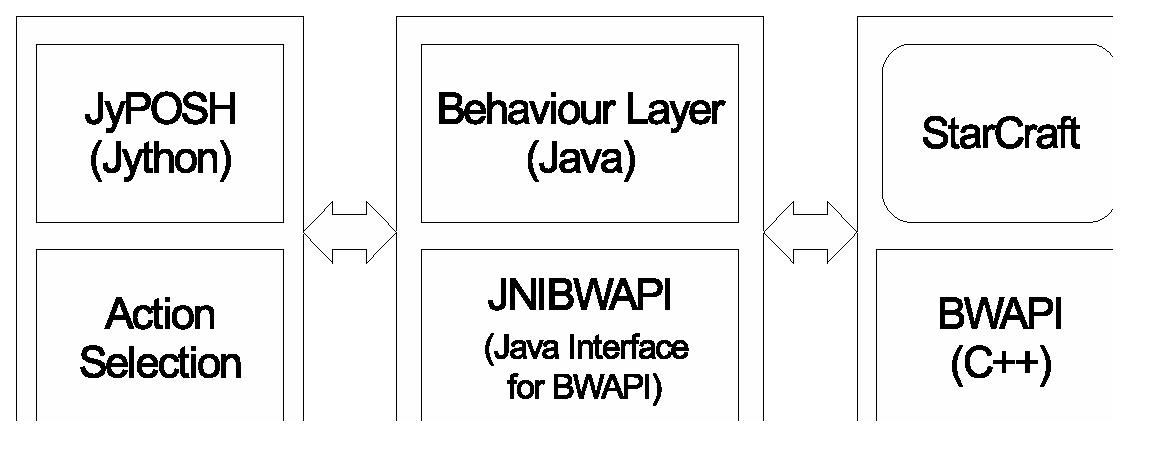
\includegraphics[scale=0.5]{AIArch}
    \caption{The architecture model for the StarCraft BOD AI. \protect\cite{davies2012}}
    \label{fig:AI-Architecture}
\end{figure}

The architecture is slightly more complicated than it needs to be, but Davies had trouble linking the python of POSH to the C++ used by BWAPI, so Java is used as an intermediary. Simplifying the architecture of the project now would require a major re-write and possibly a re-implementation of POSH in C++. This is outside the goal and scope of this project and in no way necessary, as long as JNIBWAPI remains up-to-date with BWAPI.

\label{LitSrvyClass}
The Java behaviour library of the bot is implemented as a collection of managers, which split the behaviours into correlated sub-sections. The decomposition Davies chose appears effective and his reasoning is solid.  Most of the behaviours and the action patterns are specific to the Zerg race, and as mentioned above, the other races do play quite differently. However, the base mechanics of the game (resource gathering, construction, research) are nearly identical between races and it is these areas I will look to generalise.

\section{Possible ideas for expansions}
This section covers recent AI strategies implemented for StarCraft and offers some opinion on their applicability for improving Simon's bot.

\subsection{Unit micro-management strategies}
Unit micro-management (micro) refers to the low-level control of units; how the units are positioned, what the units attack, and how the units attack \cite{TLMicro}.
The micro of Davies' bot is relatively simple compared to some other examples. There is a single army that moves towards the enemy's base. Each unit prioritises visible enemies based on their type and how far away they are. Each unit will then attack the unit it calculates to have the highest priority. While simple, this can be effective in some situations. It does have problems, units don't make use of any abilities they possess and units don't consider their position, so a weak ranged unit can end up in melee range. There are other works that show possible paths for improvement.

\subsubsection{Potential fields}
Adapted from an idea in physics, this is where individual entities in the game are given an attractive or repulsive force. So your units would be attracted to weak units while being repulsed from stronger or more dangerous units. Units can also be affected by changes in their own circumstances, perhaps retreating while under fire. The advantage of potential fields is that a single function can control lots of units, however the strength of the forces involved must be figured out manually (though someone has used genetic algorithms to improve theirs \cite{rathe2012micromanagement}). The Berkeley Overmind \cite{BerkeleyOvermind} implemented potential fields to such success that it was able to beat an ex-professional player \cite{OvermindArticle}. There are also an open source implementation available \cite{AIBot}.

\subsubsection{Monte-Carlo planning}
Planning is usually associated with large scale strategy, due to its time cost and the large search space of micro-management. Wang et al \cite{zheusing} have used a Monte-Carlo planning method. Monte-Carlo methods rely on entering random samples into a simulation and analysing the results \cite{MonteCarlo}. Wang et al created a simulation of the game state and then evaluated several predefined stochastic plans. They tested their AI in game and an imbalanced scenario (their AI was at a disadvantage) and it was able to beat beginner players and the original AI with some consistency, though was still beaten by an expert. This does show some potential for planning at a micro level, but there are problems related to the speed of the simulation and the amount of expert knowledge needed to create the plans. They haven't made their implementation public, so it's unlikely this could be integrate into Simon's bot.

\subsubsection{Bayesian Modelling}
There is a project that focuses on using Bayesian models for all aspects of a StarCraft AI \cite{synnaeve2012bayesian} which includes unit control \cite{synnaeve2011bayesian}. This uses the distribution of game elements to decide what to do with a unit next. Units receive tactical goals as sensory inputs and maintain a finite state machine (FSM) for different modes (attacking, defending, etc.). It uses re-enforcement learning to build its probability tables and succeed quite well in trails against both the original AI and against winners of the 2010 AIIDE competition. Their implementation is available open source.

\subsection{Macromanagement strategies}
Macromanagemt (macro) as used in computer gaming is a term for the economic or large-scale strategy of the player. For StarCraft, this covers resource collection, and the decision on what to build. Davies' bot is quite effective on the resource collection side, but is very restricted on the 'what to build' side. Its strategy is very rigid and doesn't adapt to the enemies actions, which is a key part of successful StarCraft play. Improving and generalising his work will require creating several strategies, and should look into making them adaptable. There is work done in StarCraft in this area.

\subsubsection{Micro Focus}
Safadi and Ernst \cite{safadi2010organization} take the interesting position that a bots macro strategy is fairly unimportant. Their view is that planning and pattern recognition is something humans excel so well at that a bot couldn't hope to match it, the bot would require a database of possible strategies which would require continuous updates as the meta-game evolves. Instead the bot should play to it's advantages in the multi-tasking area; 300 unique action per minute is considered the average for StarCraft professionals, but it would be trivial for a computer to match and beat that. They did have some success and this is comparable to how the Berkeley Overmind succeeds. However, StarCraft units generally have a "Rock Paper Scissors" dynamic; they are strong against some units and are countered by others. Effective unit-level play needs effective unit choice otherwise it can be easily exploited.

\subsubsection{Planning}
There are many replays of StarCraft games publicly available \cite{Replays}, some of which are of high level play. Using BWAPI, it's possible to retrieve lots of data from these replays and data mine the results. There are several papers that do this and use the data to create Bayesian models of what the opponents are likely to be doing \cite{synnaeve2011bayesian,hostetler2012inferring,weber2009data}.  This has the advantage that the bot gains expert-level knowledge without its creator needing to know expert strategies and it also has quite a low operational footprint. Planning and prediction seem to be popular in the StarCraft AI field, probably due to the availability of vast amounts of completed game data.

\subsubsection{Case-based reasoning}
Certicky \cite{certicky2013case} implemented cased-based reasoning (CBR) for army composition. CBR is a cyclical process where there is a databases of problem cases with solutions. For each problem, a case is chosen that best fits. The solution is adapted to fit the current problem and if it works it is added back to the database as a new case. Certicky constructed his cases based on the ratios of units that the opponent has and the solutions are the recommend ratios for the bots army. This process has the potential to be useful, but it needs quite a bit of expert knowledge about common army ratios and their counters. Additionally, this relies on good scouting and accurate information, if the bot picks the wrong case it could be disastrous.



%%
%% NOTE: Replace the following with chapters that are appropriate for your
%%       style of project.  It is unlikely these will fit your project perfectly.
%%

\chapter{Requirements}
If you are doing a primarily software development project, this is the
chapter in which you review the requirements decisions and
critique the requirements process.


Not many requirements to add

\section{Functional Requirements}
\begin{itemize}
\item An agent must be able to control the Protoss race:
    \begin{itemize}
    \item{Must be able to gather resources as the Protoss}
    \item{Must be able to create Protoss units and buildings}
    \item{Must be able to attack the enemy as the Protoss}
    \end{itemize}
\item An agent must be able to control the Terran race:
    \begin{itemize}
    \item{Must be able to gather resources as the Terran}
    \item{Must be able to create Terran units and buildings}
    \item{Must be able to attack the enemy as the Terran}
    \end{itemize}
\end{itemize}
\section{Non-Functional Requirements}
\begin{itemize}
\item{The behaviour library refactoring should not negatively affect the existing Zerg agent's performance.}
\item{The behaviour library should avoid race specific behaviour where possible}
\end{itemize}

\section{Inherited Non-Functional Requirements}
Davies' \cite{davies2012} specified several non-functional requirements that are still relevant to the project.
\begin{itemize}
\item{The application must use the BWAPI interface for communicating with StarCraft}
\item{The agent must be able to work in the latest version of StarCraft: Brood War}
\item{The AI should be designed in a modular and extensible fashion, to allow for future developments and improvements}
\item{The application must be able to run at a minimum of speed of a frame every 42ms, so not to slow down the game, as specified by the current AIIDE rules.}
\item{All relevant AI behaviours must be accessible to the POSH action selection mechanism}
\end{itemize}


\chapter{Design}

\section{Initial Structure}

The behaviour library is the main place that needs to be refactored and generalised. As mentioned in \ref{LitSrvyClass}, the behaviour library is decomposed into eight classes which manager the different areas of the game. Davies' class diagram can been seen in \ref{fig:SimonClassDia} and he outlined the class thusly:
\begin{description}
\item[Resource Manager]{Senses for actual and predicted resource counts, as well as reserving resources for future building construction.}
\item[Unit Manager]{Allows the selection of specific unit types. Mostly used by other managers.}
\item[Worker Manager]{Keeps track of workers and holds the behaviour for collecting minerals and gas. Used by the building manager for accessing workers for construction purposes.}
\item[Intelligence Manager]{Holds a knowledge base of enemy locations, and sends units to gather intelligence on enemy positions.}
\item[Building Manager]{Allows for construction of new buildings. Calculates viable building locations, and also holds senses for which buildings are currently possessed by the player.}
\item[Production Manager]{Behaviours for the creation of new units.}
\item[Upgrade Manager]{Behaviours for researching upgrades for units.}
\item[Military Manager]{Behaviours for the movement of military forces. This includes attacking the opponents base, retreating, and contains a list of priority targets.}
\end{description}

\begin{figure}[h]
    \centering
    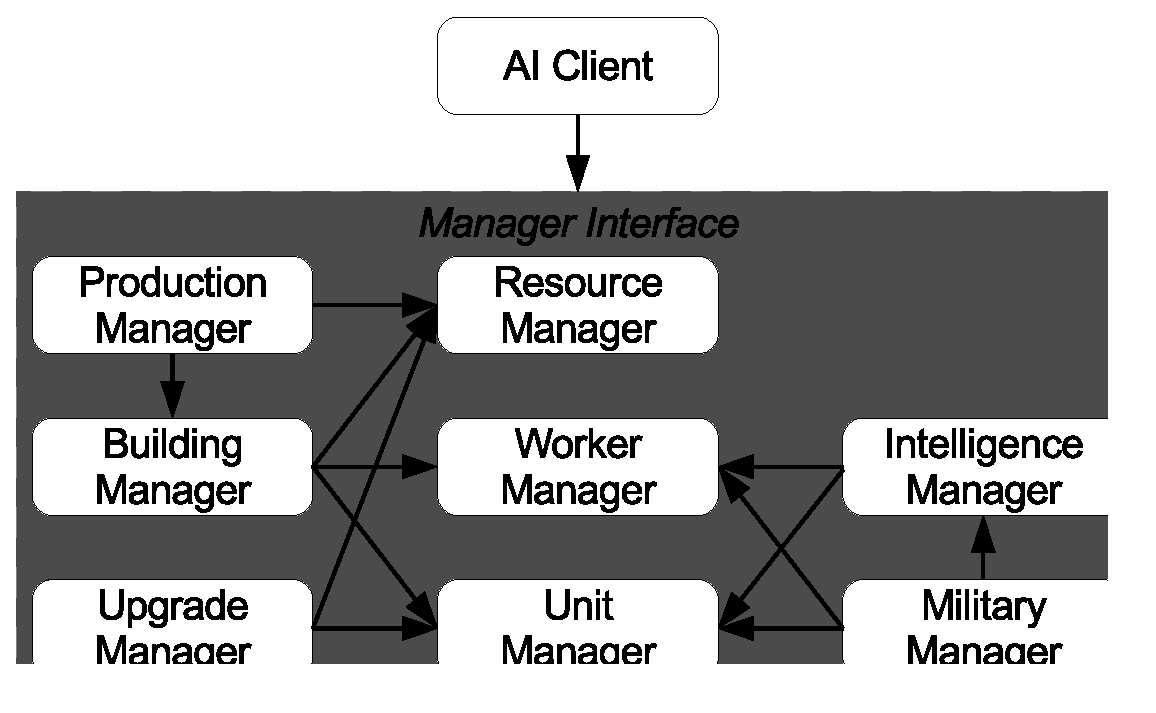
\includegraphics[scale=0.5]{OrigClassDia}
    \caption{Davies' class diagram that shows the Managers used for the categorising the different behaviours. The connections between the managers shows which classes call behaviours from other managers.\protect\cite{davies2012}}
    \label{fig:SimonClassDia}
\end{figure}


Some initial work was required to start implementing other
race's behaviours. Each manager was evaluated to identify
methods that could be generalised, and those methods that
could not be generalised were moved into a race specific
sub-class. I then followed the methodology laid out by BOD
where I would:
\begin{itemize}
\item{Implement and test simple behaviours for the other races.}
\item{Evaluate race specific behaviours, looking for common patterns that could be made general.}
\item{Implement and test generalisation.}
\item{Repeat the process.}
\end{itemize}

\chapter{Implementation and Testing}
This is the chapter in which you review the implementation and testing
decisions and issues, and critique these processes.

Code can be output inline using \verb@\lstinline|some code|@.  For example,
this code is inline: \lstinline|public static int example = 0;|  (I have
used the character \verb@|@ as a delimiter, but any non-reserved character
not in the code text can be used.)

Code snippets can be output using the \verb|\begin{lstlisting} ... \end{lstlisting}|
environment with the code given in the environment.  For
example, consider listing \ref{Example-Code}, below.

\begin{lstlisting}[breaklines,breakatwhitespace,caption={Example code},label=Example-Code]
public static void main() {

  System.out.println("Hello World");

}
\end{lstlisting}

Code listings are produced using the package ``Listings''.  This has many
useful options, so have a look at the package documentation for further
ideas.


\chapter{Results}
This is the chapter in which you review the outcomes, and
critique the outcomes process.  You may include user evaluation here
too.


%%
%% Now we are back to the standard project contents that you should include
%%

\chapter{Conclusions}
%% Uncomment this to include a separate tex file wih the conclusion contents
%\include{conclusion.tex}

This is the chapter in which you review the major achievements in the
light of your original objectives, critique the process, critique your
own learning and identify possible future work.

\bibliography{LitRef}

\appendix

%%
%% Use the appendix for major chunks of detailed work, such as these. Tailor
%% these to your own requirements
%%

\chapter{Design Diagrams}

\chapter{User Documentation}

\chapter{Raw results output}

\chapter{Code}

%%
%% NOTE that for this to typeset correctly, ensure you use the pdflatex
%%      command in preference to the latex command.  If you do not have
%%      the pdflatex command, you will need to remove the landscape and
%%      multicols tags and just make do with single column listing output
%%

\begin{landscape}
\begin{multicols}{2}
\section{File: yourCodeFile.java}
\lstinputlisting[basicstyle=\scriptsize]{yourCodeFile.java}
\end{multicols}
\end{landscape}

\end{document}